\documentclass[cs4size,a4pape,UTF8]{ctexart}   
%==================== 数学符号公式 ============
\usepackage{amsmath}                 % AMS LaTeX宏包
\usepackage[style=1]{mdframed}
\usepackage{amsthm}
\usepackage{amsfonts}
\usepackage{mathrsfs}                % 英文花体字 体
\usepackage{bm}                      % 数学公式中的黑斜体
\usepackage{bbding,manfnt}           % 一些图标,如 \dbend
\usepackage{lettrine}                % 首字下沉,命令\lettrine
\def\attention{\lettrine[lines=2,lraise=0,nindent=0em]{\large\textdbend\hspace{1mm}}{}}
\usepackage{longtable}
\usepackage[toc,page]{appendix}
\usepackage{geometry}                % 页边距调整
\geometry{top=3.0cm,bottom=2.7cm,left=2.5cm,right=2.5cm}
%====================公式按章编号==========================
\numberwithin{equation}{section}
\numberwithin{table}{section}
\numberwithin{figure}{section}
%================= 基本格式预置 ===========================
\usepackage{fancyhdr}
\pagestyle{fancy}
\fancyhf{}  
\fancyhead[C]{\zihao{5}  \kaishu Beijing University of Posts and Telecommunications}
\fancyfoot[C]{~\zihao{5} \thepage~}
\renewcommand{\headrulewidth}{0.65pt} 
\CTEXsetup[format={\centering\bfseries\zihao{2}}]{section}
\CTEXsetup[nameformat={\bfseries\zihao{3}}]{subsection}
\CTEXsetup[nameformat={\bfseries\zihao{4}}]{subsubsection}
%================== 图形支持宏包 =========================
\usepackage{subfigure}
\usepackage{graphicx}                % 嵌入png图像
\usepackage{color,xcolor}            % 支持彩色文本、底色、文本框等
\usepackage{hyperref}                % 交叉引用
\usepackage{caption}
\captionsetup{figurewithin=section}
%==================== 源码和流程图 =====================
\usepackage{listings}                % 粘贴源代码
\usepackage{xcolor}
\usepackage{color}
\definecolor{dkgreen}{rgb}{0,0.6,0}
\definecolor{gray}{rgb}{0.5,0.5,0.5}
\definecolor{mauve}{rgb}{0.58,0,0.82}
 \usepackage{xcolor}
 \lstset{
  %行号
    numbers=left,
    %背景框
    framexleftmargin=8mm,
    frame=none,
     %背景色
    %backgroundcolor=\color[rgb]{1,1,0.76},
     backgroundcolor=\color[RGB]{245,245,244},
     %样式
   keywordstyle=\bf\color{blue},
   identifierstyle=\bf,
    numberstyle=\color[RGB]{0,192,192},
    commentstyle=\it\color[RGB]{0,96,96},
   stringstyle=\rmfamily\slshape\color[RGB]{128,0,0},
   %显示空格
    showstringspaces=false
 }


%--------------------
\hypersetup{hidelinks}
\usepackage{booktabs}  
\usepackage{shorttoc}
\usepackage{tabu,tikz}
\usepackage{float}

\usepackage{multirow}



\tabcolsep=1ex
\tabulinesep=\tabcolsep
\newlength\tikzboxwidth
\newlength\tikzboxheight
\newcommand\tikzbox[1]{%
        \settowidth\tikzboxwidth{#1}%
        \settoheight\tikzboxheight{#1}%
        \begin{tikzpicture}
        \path[use as bounding box]
                (-0.5\tikzboxwidth,-0.5\tikzboxheight)rectangle
                (0.5\tikzboxwidth,0.5\tikzboxheight);
        \node[inner sep=\tabcolsep+0.5\arrayrulewidth,line width=0.5mm,draw=black]
                at(0,0){#1};
        \end{tikzpicture}%
        }

\makeatletter
\def\hlinew#1{%
  \noalign{\ifnum0=`}\fi\hrule \@height #1 \futurelet
   \reserved@a\@xhline}
   
\newcommand{\tabincell}[2]{\begin{tabular}{@{}#1@{}}#2\end{tabular}}%

\usepackage{subfigure}

\usepackage{CJK}
\usepackage{ifthen}


\usepackage{graphicx} 
\newcommand{\HRule}{\rule{\linewidth}{0.5mm}}

\newtheorem{Theorem}{定理}
\newtheorem{Lemma}{引理} 
%%使得公式随章节自动编号
\makeatletter
\@addtoreset{equation}{section}
\makeatother
\renewcommand{\theequation}{\arabic{section}.\arabic{equation}}

%-------------------------
	
\usepackage{pythonhighlight}
\usepackage{tikz}                    
\usepackage{tikz-3dplot}
\usetikzlibrary{shapes,arrows,positioning}
%===================   正文开始    ===================
\begin{document}
\bibliographystyle{gbt7714-2005}     %论文引用格式
%===================  定理类环境定义 ===================
\newtheorem{example}{例}              % 整体编号
\newtheorem{algorithm}{算法}
\newtheorem{theorem}{定理}            % 按 section 编号
\newtheorem{definition}{定义}
\newtheorem{axiom}{公理}
\newtheorem{property}{性质}
\newtheorem{proposition}{命题}
\newtheorem{lemma}{引理}
\newtheorem{corollary}{推论}
\newtheorem{remark}{注解}
\newtheorem{condition}{条件}
\newtheorem{conclusion}{结论}
\newtheorem{assumption}{假设}
%==================重定义 ===================
\renewcommand{\contentsname}{目录}     
\renewcommand{\abstractname}{摘要} 
\renewcommand{\refname}{参考文献}     
\renewcommand{\indexname}{索引}
\renewcommand{\figurename}{图}
\renewcommand{\tablename}{表}
\renewcommand{\appendixname}{附录}
\renewcommand{\proofname}{证明}
\renewcommand{\algorithm}{算法} 
%============== 封皮和前言 =================
\begin{titlepage}

\begin{center}


% Upper part of the page

\includegraphics[width=0.65\textwidth]{figure/logo}\\[1cm]    

\textsc{\Large 论文}\\[0.5cm]


% Title
\HRule \\[1.5cm]
{ \huge \bfseries 形式化分析介绍}\\[0.94cm]
\HRule \\[1.5cm]

% Author and supervisor
\begin{minipage}{0.4\textwidth}
\begin{flushleft} \large
\emph{姓名: }
 \textsc{冯皓楠}\\
\end{flushleft}
\end{minipage}
\begin{minipage}{0.4\textwidth}
\begin{flushleft} \large

\end{flushleft}

\end{minipage}

\vfill

% Bottom of the page
{\large \today}

\end{center}

\end{titlepage}


%%=============设计(论文)任务书===========
%\begin{center}
%\zihao{-2}\textbf{\songti 本科生毕业设计(论文)任务书} 
%\end{center}
%\smallskip
%\renewcommand{\arraystretch}{1.3}
%\begin{tabular}{lll}
%\zihao{4} \textbf{\songti 学生姓名: 曹宇} & & \zihao{4} \textbf{\songti 专业班级:\quad\quad 船海1006班} \\ 
%\zihao{4} \textbf{\songti 指导教师:徐海祥}&\makebox [3cm] & \zihao{4} \textbf{\songti 工作单位:\quad 武汉理工大学} \\ 
%\end{tabular}\\
%\begin{tabular}{lll}
%\zihao{4} \textbf{\songti 设计(论文)题目:}& \zihao{4} \textbf{\songti  武汉理工本科论文\LaTeX 模板 } &\\ 
%\zihao{4} \textbf{\songti 设计(论文)主要内容:} \\
%\end{tabular} \\ 
%\begin{enumerate}
%\item \LaTeX 环境的配置
%\item 主要字体的控制和数学公式的选用
%\item 图表和代码的粘贴
%\end{enumerate}
%\begin{tabular}{ll}
%\zihao{4} \textbf{\songti 要求完成的主要任务:}
%\end{tabular} \\ 
%\begin{enumerate}
%\item 选择合适的\TeX 编辑系统
%\item 学习如何使用控制代码完成排版
%\item 合理的安排学习和科研的时间来发展自己兴趣爱好
%\end{enumerate}
%\begin{tabular}{ll}
%\zihao{4} \textbf{\songti 必读参考资料:}
%\end{tabular}
%\begin{enumerate}
%\item \LaTeX  \quad User Manual
%\item  字体设计的艺术
%\end{enumerate}
%\begin{tabular}{lll}
%\zihao{4} \textbf{\songti 指导教师签名: }&\makebox [4cm]& \zihao{4} \textbf{\songti 系主任签名:} \\
%& & \zihao{4} \textbf{\songti 院长签名(章)}
%\end{tabular}
%\thispagestyle{empty}
%\clearpage
%%==========本科生毕业设计(论文)开题报告  =============
%\begin{center}
%\zihao{-2} \textbf{\songti 武汉理工大学}\\
%\zihao{-2} \textbf{\songti 本科生毕业设计(论文)开题报告} 
%\end{center}
%\begin{tabular}{|l|}
%\hline \rule[-2ex]{0pt}{5.5ex} \makebox[13.5cm][l]{\zihao{4} \heiti 1、目的及意义(含国内外的研究现状分析) } \\ 
%\quad \LaTeX 是国际通行的科技论文排版软件,国际上科研机构和大学都采用它写作\\
%\quad 国内著名高校都有自己的本科生\LaTeX 模板供毕业生使用\\
%\quad 但是武汉理工大学还没有本科生\LaTeX 模板可以参考\\
%\quad 人类的价值在于创造而不是索取 \\
%\hline \rule[-2ex]{0pt}{5.5ex}  \zihao{4} \heiti
%2、基本内容和技术方案\\ 
%\quad 采用GITHUB托管降低代码维护成本\\
%\quad 加入在线\TeX 编辑器的使用简介 \\
%\quad 授人以渔,注重方法和理念的引导\\
%\hline \rule[-2ex]{0pt}{5.5ex}  \zihao{4} \heiti
%3、进度安排 \\ 
%\quad 离 deadline 两个月吃喝玩乐 \\
%\quad 离 deadline 一个月吃喝玩乐 \\
%\quad 离 deadline 半个月吃喝玩乐 \\
%\quad 离 deadline 一个星期狂写论文 \\
%\hline \rule[-2ex]{0pt}{5.5ex} \zihao{4} \heiti
%4、指导教师意见 \\ 
%\quad 曹宇同学是个好同志\\
%\quad 曹宇同志是个好同学\\
%\quad 本表格是支持跨页的长表格,你可以复制上面的内容进行测试\\
%\quad 具体方法是将tabular改为 longtable然后再编译\\
%\makebox[10cm][r]指导教师签名:\\
%\makebox[12cm][r]\quad 年\quad 月\quad 日\\
%\hline 
%\end{tabular} 
%\thispagestyle{empty}

\pagestyle{plain}
\pagenumbering{Roman}

\section*{\zihao{2} \centering \textbf{摘要} }

\vskip0.5cm

形式化方法是基于数学的特种技术,适合于验证和设计。形式化方法适用的领域非常多,除了在数学领域的机器证明,形式化方法还可以应用在计算机领域的硬件与软件验证,安全协议领域的协议验证与协议设计。将形式化方法用于软件和硬件设计,是期望能够像其它工程学科一样,使用适当的数学分析以提高设计的可靠性和鲁棒性。将形式化应用于安全协议分析,通过数学的手段可以发现人无法发现的协议漏洞,还可以证明协议在某些方面的安全性。

本文综合了与形式化、形式化方法、形式化分析、形式化验证有关的论文与网络资源内容,对与形式化应用的领域做了简单的介绍,并详细总结了形式化方法在安全协议领域的应用与方法。

\textbf{关键词:}  形式化方法,形式化验证, 安全协议 的形式化分析 


\addcontentsline{toc}{section}{摘要}





\pagestyle{empty}
\tableofcontents 
\thispagestyle{empty}
%============== 论文正文   =================
\pagestyle{fancy}
\newpage
\pagenumbering{arabic}%开始数字目录
\section{介绍}
 本章用于介绍与形式化有关的名词含义。
 
\subsection{形式化方法(Formal Methods)}
形式化方法是将概念或方法,经过高度抽象后使用一定的数学模型进行表示。之后,通过程式化的推演和计算来研究该数学模型,进而揭示概念和方法内在规律的一种研究方法。

形式化方法简单的说就是用数学工具进行定义、开发和验证(specification, development and verification)。数学家们认为,不论硬件还是软件工程,就像世间万物一样,所有的学问一样,归根结底是数学问题。''一个不懂数学的工程师不是一个好工程师''。如果所有的设计开发都能够按照严格的数学方法进行,那么开发出来的系统就会像数学本身一样的完美:软件不会出错,硬件永远正常。当然,这是数学家的理想。

来自维基百科(Formal method):在计算机科学中,特别是软件工程和硬件工程中,形式化方法是一种特殊的基于数学的技术,用于软件和硬件系统的规范、开发和验证。软件和硬件设计的形式化方法的产生于使用是由于用户对安全性不断上涨的期望导致的,像在其他同城学科一样,执行适当的数学分析可以提高设计系统的可靠性和健壮性。

In computer science, specifically software engineering and hardware engineering, formal methods are a particular kind of mathematically based techniques for the specification, development and verification of software and hardware systems. The use of formal methods for software and hardware design is motivated by the expectation that, as in other engineering disciplines, performing appropriate mathematical analysis can contribute to the reliability and robustness of a design。

Formal methods are best described as the application of a fairly broad variety of theoretical computer science fundamentals, in particular logic calculi, formal languages, automata theory, discrete event dynamic system and program semantics, but also type systems and algebraic data types to problems in software and hardware specification and verification。

当代著名逻辑学家鲍亨斯基认为:"形式化方法是这样一种方法,它完全撇开符号本身的意义,而根据某些只涉及符号书面形态的转换规则来进行符号操作的方法。
理解''形式化方法''时,注意区分与软件形式化方法(软件可靠性方法),因为形式化方法在软件工程领域的应用比较广泛,所以形式化方法往往指代软件形式化方法,即软件工程中的形式化设计与形式化验证等。


\subsection{形式化规范}
形式化规范就是用一套基于明确定义的数学概念的符号来书写,并且通常伴随着支持性的解释(非形式化)语句。这些数学概念被用来定义符号的句法和语义,以及支持逻辑推理的证明规则。支持形式化符号的句法和语义规则应该定义如何明确地识别其结构和确定其含义。并且必须有证据表明矛盾不可能产生,支持符号的所有规则都有定义或者引用。

\subsection{形式化语言}
使用的是以数学、数理逻辑符号语言为蓝本的科学语言,也称为"形式化语言"。它的基本特征是:语言保持单一性、无岐义性和明确性。形式化语言的推广运用作为一种用于研究手段,被称为形式化方法。

\subsection{形式化验证(Formal Verification)}
形式化验证(又叫形式化证明),在数学,计算机科学,人工智能领域都得到了广泛的应用。形式化的概念最早出现在数学界,又称为机器证明。

CertiK(一个用形式化验证为智能合约和区块链应用提供安全性服务的公司)的创始人顾荣辉用简洁的语句来描述形式化验证:用逻辑语言来描述规范,通过严谨的数学推演来检查给定的系统是否满足要求。

来自维基百科(Formal Verification):在硬件和软件系统中,形式化验证是通过形式化的数学方法来证明一个系统潜在算法的正确性行为或否定一个系统潜在算法的正确性行为。形式化验证可以帮助证明系统的正确性,例如:加密协议、组合电路、带有内部内存的数字电路,以及源代码形式表示的软件。对于这些系统的验证是通过对系统的抽象数学模型的形式化证明、数学模型与系统的性质之间的对应关系来实现的。通常用于建模系统的数学对象有有限状态机、标记转换系统、向加法系统、自动机、过程代数、编程语言的形式化语义等。

In the context of hardware and software systems, formal verification is the act of proving or disproving the correctness of intended algorithms underlying a system with respect to a certain formal specification or property, using formal methods of mathematics.

Formal verification can be helpful in proving the correctness of systems such as: cryptographic protocols, combinational circuits, digital circuits with internal memory, and software expressed as source code.

The verification of these systems is done by providing a formal proof on an abstract mathematical model of the system, the correspondence between the mathematical model and the nature of the system being otherwise known by construction. Examples of mathematical objects often used to model systems are: finite state machines, labelled transition systems, Petri nets, vector addition systems, timed automata, hybrid automata, process algebra, formal semantics of programming languages such as operational semantics, denotational semantics, axiomatic semantics and Hoare logic.


\section{形式化方法在不同领域的应用}
形式化方法的应用主要如下:

\begin{itemize}
\item 安全模型
\item 流分析
\item 安全协议分析
\item 软件验证
\item 硬件验证
\item 体系结构分析
\item 秘密信道分析
\end{itemize}

\subsection{数学领域的形式化}
数学领域,形式化的工作主要在于机器验证数学定理。
定理证明器包含Coq、Z3、CVC4、Vampire、E、Spass、Isabelle证明器等。以下是一个在Isabelle定理证明器中,关于质数的平方根不是有理数的证明:

\begin{figure}[thbp!]
\centering
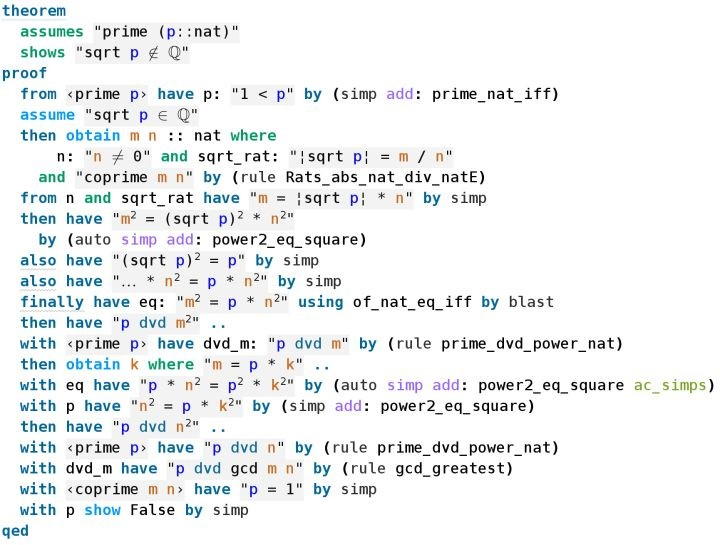
\includegraphics[width=0.6\linewidth]{figure/1}
\caption{Isabelle证明器验证数学定理}
\label{fig:1}
\end{figure}
 
但是,由于数学定理的形式化证明因其过度的复杂性和晦涩的机器表达力,

\subsection{计算机领域的形式化}
\subsubsection{硬件设计领域}
形式化方法在计算机领域是从硬件设计开始普及的,一个例子:当年Intel的Pentium CPU浮点运算单元出错(FDIV Bug),数以万计的CPU不得不回收和替换,给Intel造成了巨大损失(475M美元)。从那之后,Intel开始在其芯片设计中广泛采用形式化方法。

\subsubsection{软件可靠性方法}
形式化方法在计算机领域最常用的就是软件工程中的形式化方法,又称软件可靠性方法,一般提起形式化方法,往往指的就是计算机领域的软件形式化方法。

从广义上讲,形式化方法是借助数学的方法来解决软件工程领域的问题,主要包括建立精确的数学模型以及对模型的分析活动。狭义的讲,形式化方法是运用形式化语言,进行形式化的规格描述、模型推理和验证的方法。就形式化建模而言,形式化表示必须包含一组定义其语法语义的形式化规则。这些规则可用于分析给定的表达式是否符合语法规定,或证明该表达式具有某种性质。

形式化方法的出发点是数学逻辑方法,其目的是开发可靠的软件产品。从软件开发来讲,形式化方法目前并非软件开发的主流。从软件发展看,早期的软件是用于数值计算,程序语言侧重于函数和算法的描述,后来数据库的应用和数据结构逐渐变得重要。现在的软件更为复杂,因此,对象、组件、接口、通讯、开放等成为非常重要的概念。从软件工程方法来讲,有一套描述这些概念的办法,比如说用图形、表格、逻辑、自然语言等,交叉使用以描述一个系统的各个方面。因此换一个角度来考虑,我们也可以以目前常用的软件开发方法为出发点,研究怎样将这些方法形式化,使软件系统的描述精确化,以减少可能的误解所带来的问题;或以目前常用的软件开发过程为出发点,研究怎样在软件开发过程中增加一些形式化方法的应用,以提高软件的可靠性。

\subsection{协议领域的形式化}
安全协议的形式化分析主要包含:

\begin{itemize}
\item 安全协议的形式化验证(formal verification)
对已经存在的安全协议进行验证,判断这些安全协议是否达到预期的目标。
\item 安全协议的形式化设计(formal design)
从无到有,设计出安全的协议。
\end{itemize}

\newpage
\section{安全协议的形式化分析方法}
安全协议的形式化分析从方法上可以分为:逻辑推理、模型检测、定理证明。

\subsection{逻辑推理}
逻辑推理是基于知识与信念推理的分析方法,主要运用逻辑系统从用户接受和发送的消息出发,通过一系列的推理公推证协议是否满足安全规范。

模态逻辑方法是分析安全协议最直接,最简单的一种方法。

1989年,Burrows,Abadi和Needham提出了著名的BAN逻辑,这种逻辑利用知识和信念逻辑来描述和推理认证协议,通过协议理想化、初始嘉定确定、断言确定和逻辑推理等步骤,验证协议的人整形目标。它简单,直观,便于掌握和使用,是安全协议形式化分析研究中的一个重要的里程碑。

但是,BAN逻辑也有缺陷,它的语义不够精确、协议理想化和初始假设的确定非形式化、推理规则不够完备等,只能验证认证性质,不能认证机密性等其他安全性之。

为了克服BAN逻辑的不足,之后又出现多种BAN类逻辑,如GNY、AT、VO、SVO和MB等逻辑,这些扩展的BAN类逻辑语义更加精确,且根据具体使用情况,学者们还提出了一些专用逻辑,用于分析特定的协议,使这种方法能够支持复杂的安全协议验证,能够检测BAN逻辑无法检测的攻击,应用十分广泛,但都没有原始的BAN逻辑简单实用。

下面介绍BAN逻辑的基本原理。

BAN逻辑的推理步骤: 
\begin{itemize}
\item 用逻辑语言对系统的初始状态进行描述
\item 建立理想化的协议模型,将协议的实际消息转换成BAN逻辑能识别的公式
\item 对协议进行解释,将协议转换为逻辑语言
\item 应用逻辑的推理规则根据理想化协议和假设进行推理,推断协议能否完成预期的目标。如果在协议流程结束时能够建立关于共享密钥、对方身份等知识与信念的信任,则表明协议是安全的;反之,表明协议存在安全漏洞。
\end{itemize}

BAN逻辑的基本模型如图(\ref{fig:3})所示。

\begin{figure}[h!]
\centering
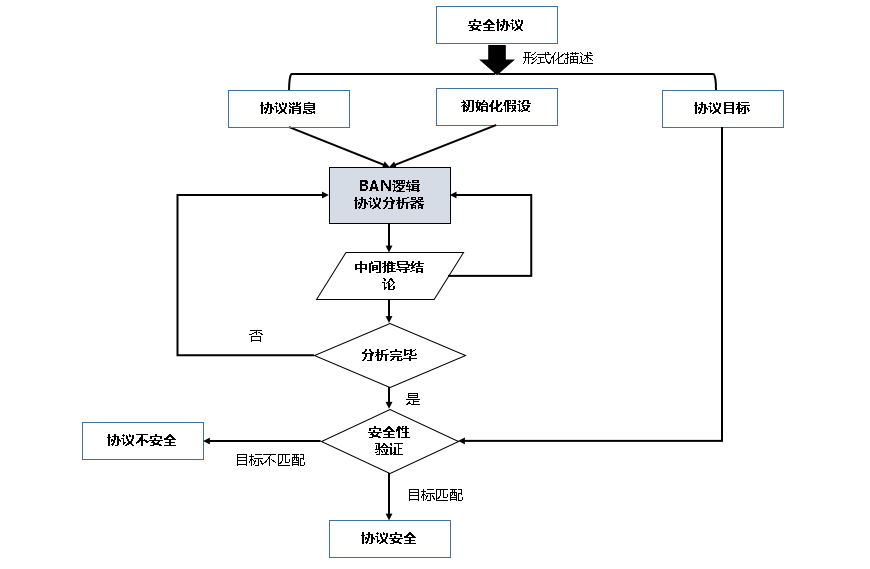
\includegraphics[width=0.6\linewidth]{figure/3}
\caption{BAN逻辑的基本模型}
\label{fig:3}
\end{figure}

BAN逻辑的推理规则有:

\begin{itemize}
\item 消息含义规则
\item 随机数验证规则
\item 临时值验证规则
\item 仲裁规则
\item 信仰规则
\item 发送规则
\item 接收规则
\item 共享密钥规则
\item 共享秘密规则
\end{itemize}

消息含义规则如下图表示:

\begin{figure}[thbp!]
\centering
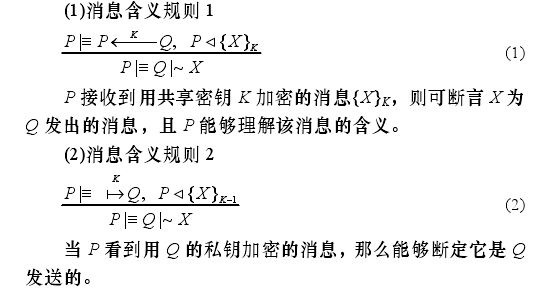
\includegraphics[width=0.6\linewidth]{figure/2}
\caption{消息含义规则示例}
\label{fig:2}
\end{figure}

这种方法的不足主要表现在它逻辑的抽象级别较高,分析范围过窄,不能对知识进行推理,只能分析协议的认证性质,只能发现协议的缺陷,不能保证协议一定是安全的。

\subsection{模型检测(model checking)}
模型检测最早用于分析和模拟硬件的工作过程。1996年,Gavin Lowe首次将模型检测器FDR用于安全协议的验证,结合CSP安全协议模型成功发现了针对NSPK协议的攻击,伺候,又出现了NRL,Interrogator,CSP/FDR,Brutus,SMV,MUφ,SPN,Athena,OFMC,SATMC等大量自动化验证器。

模型检测主要通过状态空间搜索方法来检测协议安全性,其基本思想是将安全协议看做包含一个状态集合、一个动作集合、一个状态转移集合的分布式系统。协议的执行过程就是状态的迁移过程,协议验证就是遍历整个状态空间,检查是否能由初试的状态到达某个不安全状态或者可以引发某个不良行为的状态。初始状态到最终状态之间的所有状态构成了一个协议执行轨迹,如果一个协议不安全,就可以通过协议迹给出相应的反例。

对于该方法面临的''状态空间爆炸问题'',可以通过控制状态空间大小,控制搜索过程的手段来解决。不同的模型检测器都有着相关的技术来解决这一问题。

对于目前的协议分析来讲,模型检测已经证明是一条非常成功的途径,这种方法的自动化程度高,验证过程不需要用户参与,而且如果协议有缺陷,能够自动产生反例,但是缺点也很明显,就是容易产生状态空间爆炸,一般需要制定运行实例和主体数量等运行参数。同时,在无限状态模型中,模型检测无法完全确定协议是安全的。

\subsubsection{通用模型检测器}
通用模型检测器有FDR、SPN、SMV等。

在建模入侵者模型是,需要规定入侵者知道和不知道的消息,如果消息的数目是无限的,则模型本身也将是无限大的,这样在模型中就必须明确规定哪些信息包含、哪些信息排除,用户的负担是简历一个入侵者的有限状态机描述,这一步相对来说比较复杂,特别是在考虑不同协议之间交互的时候。

\subsubsection{专用模型检测器}
专用模型检测器有NRL、BRUTUS等。

专用模型检测器从模型中分离出入侵者,用户不需要事先规定入侵者必须知道的消息,就可以进行协议验证。但是,专用模型检测器的简约技术不如通用模型检测器,在验证复杂协议时经常由于状态爆炸的问题而难以得到验证结果,或者验证结果过给出的反例过于复杂,难以构建攻击路径。其次,专用模型检测器通常只适用于验证某一类型的协议,或者在描述协议的某些性质和验证协议的某些阶段工作做的较好,而在其他方面则存在明显的缺陷。


\subsection{定理证明}
基于定理证明的安全协议分析方法不关注针对协议的攻击,其目的只在于证明安全协议是否满足响应的安全属性。

定理证明的分析方法解决了基于逻辑推理方法不能解决保密性验证,缺乏清晰语义的缺点,还解决了模型检测技术很难解决状态空间爆炸的缺点,可以处理不受限会话数目和不受限消息大小,在此方面Pauson和Blanchet的工作最具有代表性。但是Pauson基于归纳的方法只能实现半自动的协议形式化验证,Blanchet基于归结定理证明实现了秘密性和认证性的自动化验证,其验证器可以保证终止,但是不保证完备性,有攻击误报的情况。

(归结原理:将普通形式逻辑中充分条件的推理形式符号化,并向一阶谓词逻辑推广的一种推理法则。)

\subsubsection{归纳法}
Pauson首先将归纳法应用于协议安全性证明。Isabell把协议定义为所有可能时间执行轨迹的集合,每个执行序列反映了协议主体之间可能的通信方式。它通过对路径的归纳来证明性质的成立。该工具可以用于一个任意次数的协议会话,其证明股构成与非形式化证明方法有着相同的结构,这是它的有点,但是一旦推导失败,就很难获得协议可能的漏洞,并且分析不保证会终止,且需要大量的用户干预。

\subsubsection{串空间模型(Strand-Space)}
Fabrega等人提出了串空间模型,其中协议的正确性可以表示成不同类型串之间的连接关系。正确性证明的过程首先是建立协议规范可能形成的所有串束,再根据串束中串的连接情况判断协议中的安全属性是否得到满足。

之后,Millen等人将串空间的概念和Pauson的归纳证明方法结合起来,使用归纳方法简历协议时间的执行序列,然后在这个序列上使用''补集(co-ideal)''的概念来分析攻击者的知识,来判断保密消息是否已经泄露。

在串空间模型的基础上,Guttman等人提出了反应随机数在加密条件下与身份认证之间关系的认证测试概念,基于这种认证测试机制,既可以证明认证属性,也可以设计认证协议。

Athena是Song等人开发的专用于协议验证的定理证明器,它使用一种扩展的传空间理论作为底层的计算模型,协议的安全属性由一些公式来描述,然后由Athena系统验证这些公式的正确性。它采用宽度优先搜索,若协议不正确,能及早发现攻击行为。由于该工具基于定理证明方法,用户手动状态约简的操作必不可少,并且过程较为繁琐。

\subsubsection{阶函数(Rank Functions)}
阶函数是另一种定理证明方法,它是Schneider提出的概念。

阶函数是一个把攻击者的知识和协议消息映射成整数的函数。使用阶函数可以把消息分成攻击者知道的消息和攻击者不可知道的消息两大类。协议的认证性和秘密性均基于阶函数的值来判定。

后来,Heather和Schneider又给出了一个简历阶函数的算法和推导消息阶函数值的过程,这使得阶函数的证明过程得以自动化实现。


\section{总结}
未完待续
\end{document}
%%%%%%%%%% 结束 %%%%%%%%%%